\documentclass[12pt, a4paper]{article}

\usepackage[utf8]{inputenc}
% Limit the page margin to only 1 inch.
\usepackage[margin=1in]{geometry}

%Imports biblatex package
\usepackage[
backend=biber,
style=alphabetic
]{biblatex}
\addbibresource{../../algs4e.bib}

% Enables the `align' environment.
\usepackage{amsmath}
% Provides useful environments, such as:
% - \begin{proof} ...\end{proof}
\usepackage{amsthm}
\usepackage[most]{tcolorbox}

\newtheorem*{proposition}{Proposition}

% Enables using \mathbb{}, for example \mathbb{N} for the set of natural numbers.
\usepackage{amssymb}

% Allows using letters in enumerate list environment. Use, for example:
%\begin{enumerate}[label=(\alph*)]
% ...
%\end{enumerate}
\usepackage[inline]{enumitem}

% Enable importing external graphic files and provides useful commannds, like \graphicspath{}
\usepackage{graphicx}
% Images are located in a directory called images in the current directory.
\graphicspath{{./images/}}

% Make links look better by default.
% See: https://tex.stackexchange.com/questions/823/remove-ugly-borders-around-clickable-cross-references-and-hyperlinks
\usepackage[hidelinks]{hyperref}
\usepackage{xcolor}
\hypersetup{
	colorlinks,
	linkcolor={red!50!black},
	citecolor={blue!50!black},
	urlcolor={blue!80!black}
}


% Code Listings. Source:
% https://stackoverflow.com/questions/3175105/inserting-code-in-this-latex-document-with-indentation
\usepackage{listings}
\usepackage{color}

\definecolor{dkgreen}{rgb}{0,0.6,0}
\definecolor{gray}{rgb}{0.5,0.5,0.5}
\definecolor{mauve}{rgb}{0.58,0,0.82}

\lstset{frame=tb,
	language=Java,
	aboveskip=3mm,
	belowskip=3mm,
	showstringspaces=false,
	columns=flexible,
	basicstyle={\small\ttfamily},
	numbers=none,
	numberstyle=\tiny\color{gray},
	keywordstyle=\color{blue},
	commentstyle=\color{dkgreen},
	stringstyle=\color{mauve},
	breaklines=true,
	breakatwhitespace=true,
	tabsize=3
}

\newcommand{\prob}{\text{P}}
%\newcommand{\complement}{\mathsf{c}}

% Define an environment called "ex" (for Exercise) so that I can do: \begin{ex}{1.5}...\end{ex}
\newenvironment{ex}[2][Exercise]
{\par\medskip\noindent \textbf{#1 #2.}}
{\medskip}

% Define a solution environment, similar to ex (exercise) environment.
\newenvironment{sol}[1][Solution]
{\par\medskip\noindent \textbf{#1.} }
{\medskip}

\begin{document}
	\noindent Sergio E. Garcia Tapia \hfill
	
	\noindent \emph{Algorithms} by Sedgewick and Wayne (4th edition) \cite{sedgewick_wayne}\hfill
	
	\noindent January 09, 2025\hfill 
	\section*{4.1: Undirected Graphs}
	\begin{ex}{1}
		What is the maximum number of edges in a graph with $V$ vertices and no parallel
		edges? What is the minimum number of edges in a graph with $V$ vertices, none of
		which are isolated (have degree $0$)?
	\end{ex}
	\begin{sol}
		No parallel edges means that at most one edge connects any two given nodes.
		For any vertex $v_i$, there are $V$ possible edge candidates, including $v_0$
		itself (because loops are not disallowed, we can assume they are allowed).
		Then, for $v_1$, there are $V-1$ edges allowed: one for $v_1$, and one for each
		other vertex, except $v_0$. Continuing this way, we find that there is
		a maximum of $V!$ ($V$ factorial) edges.
		
		If $V$ is even, then the minimum is $V / 2$, since we can pair all vertices.
		If $V$ is odd, it is $\lfloor V / 2\rfloor + 1$.
	\end{sol}
	\begin{ex}{2}
		Draw, in the style of the figure in the text (page 524), the adjacency lists
		built by \texttt{Graph}'s input stream constructor for the file \texttt{tinyGex2.txt}
		depicted at left (input from \texttt{tinyGex2.txt}) (see also Figure~\ref{fig:tinyGex2-graph}).
		\begin{lstlisting}[language={}]
12
16
 8  4
 2  3
 1 11
 0  6
 3  6
10  3
 7 11
 7  8
11  8
 2  0
 6  2
 5  2
 5 10
 5  0
 8  1
 4  1
		\end{lstlisting}
		\begin{figure}
			\centering
			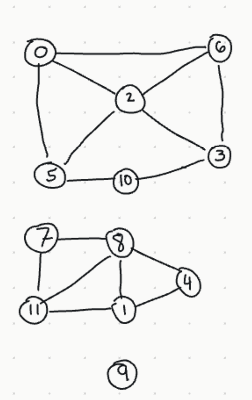
\includegraphics[width=0.2\textwidth]{exercise-02-graph}
			\caption{Graph from \texttt{tinyGex2.txt}.}
			\label{fig:tinyGex2-graph}
		\end{figure}
	\end{ex}
	\begin{sol}
		See Figure~\ref{fig:ex-02}.
		\begin{figure}
			\centering
			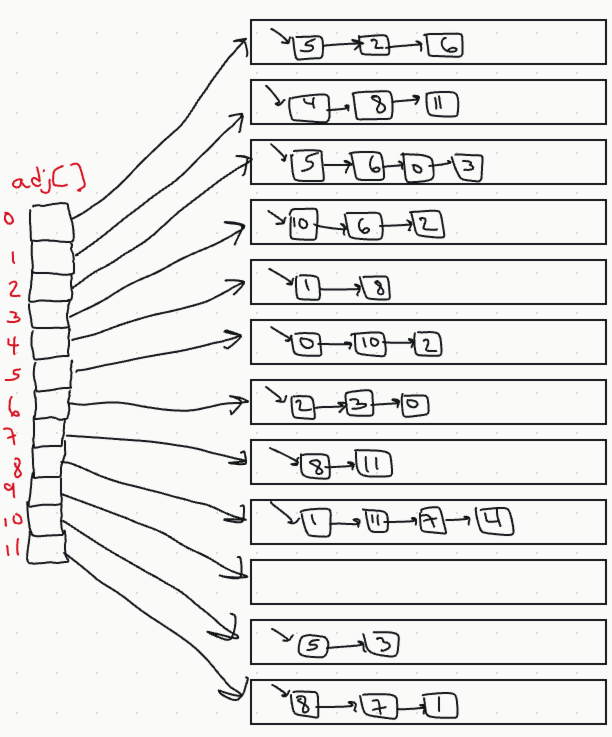
\includegraphics[width=0.5\textwidth]{exercise-02}
			\caption{Adjacency list representation for undirected graph from \texttt{tinyGex2.txt}}
			\label{fig:ex-02}
		\end{figure}
	\end{sol}
	\begin{ex}{3}
		Create a copy constructor for \texttt{Graph} that takes as input a graph
		\texttt{G} and creates and initializes a new copy of the graph. Any changes
		a client makes to \texttt{G} should not affect the newly created graph.
	\end{ex}
	\begin{sol}
		See \texttt{com.segarciat.algs4.ch4.sec1.ex03}.
	\end{sol}
	\begin{ex}{4}
		Add a method \texttt{hasEdge()} to \texttt{Graph} which takes two \texttt{int}
		arguments \texttt{v} and \texttt{w} and returns \texttt{true} if the graph has
		an edge \texttt{v-w}, \texttt{false} otherwise.
	\end{ex}
	\begin{sol}
		See \texttt{com.segarciat.algs4.ch4.sec1.ex04}.
	\end{sol}
	\begin{ex}{5}
		Modify \texttt{Graph} to disallow parallel edges and self-loops.
	\end{ex}
	\begin{sol}
		See \texttt{com.segarciat.algs4.ch4.sec1.ex05}.
	\end{sol}
	\begin{ex}{6}
		Consider the four-vertex graph with edges \texttt{0-1}, \texttt{1-2}, \texttt{2-3},
		and \texttt{3-0}. Draw an array of adjacency-lists that could \emph{not} have been
		built calling \texttt{addEdge()} for these edges \emph{no matter what order}.
	\end{ex}
	\begin{sol}
		\begin{figure}
			\centering
			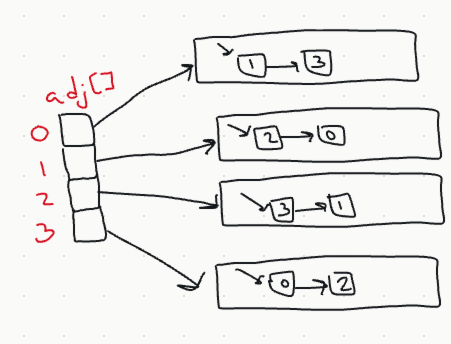
\includegraphics[width=0.3\textwidth]{exercise-06}
			\caption{Impossible adjacency-lists for a four-vertex graph with edges
			\texttt{0-1}, \texttt{1-2}, \texttt{2-3}, and \texttt{3-0}.}
			\label{fig:ex-06}
		\end{figure}
		See Figure~\ref{fig:ex-06}. The contents suggest that
		\begin{enumerate}
			\item According to 0's adjacency list, \texttt{0-3} comes before \texttt{0-1}.
			\item According to 3's adjacency list, \texttt{2-3} comes before \texttt{0-3}.
			\item According to 2's adjacency list, \texttt{1-2} comes before \texttt{2-3}.
			\item According to 1's adjacency list, \texttt{0-1} comes before \texttt{1-2}.
		\end{enumerate}
		According to the first three, the implied order is
		\begin{lstlisting}[language=java]
1-2
2-3
0-3
0-1
		\end{lstlisting}
		but then 1's adjacency list says that \texttt{0-1} comes before \texttt{1-2},
		which contradicts that \texttt{0-1} comes last in the list above. This can
		be seen from the adjacency lists because there must be first pair, which means
		that there is a pair of vertices \texttt{v} and \texttt{w} that are last in each
		other's adjacency lists. That would imply that \texttt{v-w} (or \texttt{w-v})
		was the first edge inserted. That doesn't happen in the figure, however.
	\end{sol}
	\begin{ex}{7}
		Develop a test client for \texttt{Graph} that reads a graph from the input stream
		named as command-line argument and then prints it, relying on \texttt{toString()}.
	\end{ex}
	\begin{sol}
		See \texttt{com.segarciat.algs4.ch4.sec1.ex07}.
	\end{sol}
	\begin{ex}{8}
		Develop an implementation of the \texttt{Search} API on page 528 that uses \texttt{UF},
		as described in the text.
	\end{ex}
	\begin{sol}
		See \texttt{com.segarciat.algs4.ch4.sec1.ex08}.
	\end{sol}
	\begin{ex}{9}
		Show, in the style of page 533, a detailed trace of the call \texttt{dfs(0)}
		for the graph built by \texttt{Graph}'s input stream constructor for the file
		\texttt{tinyGex2.txt} (see \texttt{Exercise 4.1.2} and Figure~\ref{fig:tinyGex2-graph}).
		Also, draw the tree represented by \texttt{edgeTo[]}.
	\end{ex}
	\begin{sol}
		From Figure~\ref{fig:tinyGex2-graph}, we see that $G$ is not connected, so
		we can focus on the connected component of $G$ that contains \texttt{0}.
		See Figure~\ref{fig:ex-09-dfs} for the race, and Figure~\ref{fig:ex-09-tree}
		for the tree.
		\begin{figure}
			\centering
			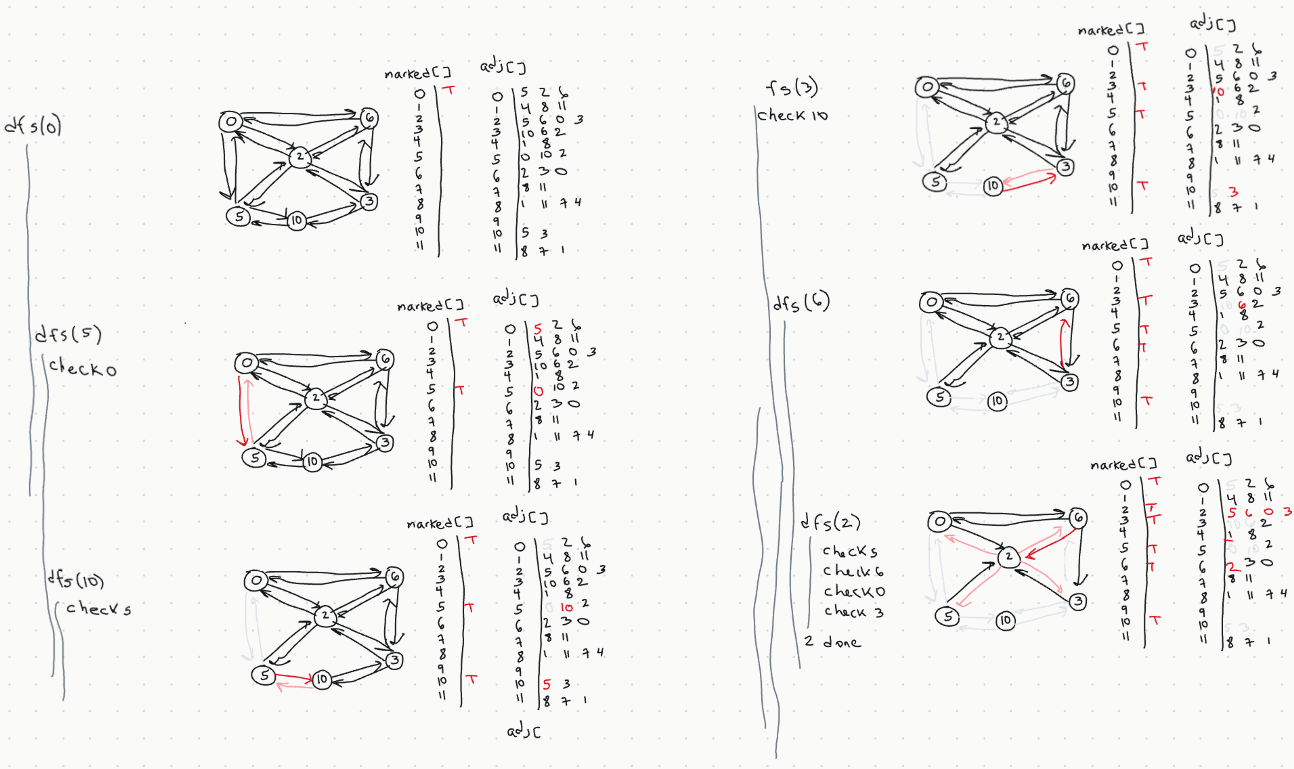
\includegraphics[width=0.9\textwidth]{exercise-09-dfs}
			\caption{Trace of depth-first search to find all paths from \texttt{0} on \texttt{tinyGex2.txt}.}
			\label{fig:ex-09-dfs}
		\end{figure}
		\begin{figure}
			\centering
			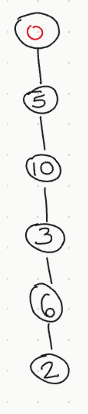
\includegraphics[width=0.05\textwidth]{exercise-09-edgeTo-tree}
			\caption{Tree built from Figure~\ref{fig:ex-09-dfs}.}
			\label{fig:ex-09-tree}
			\end{figure}
	\end{sol}
	\begin{ex}{10}
		Prove that every connected graph has a vertex whose removal (including all
		incident edges) will not disconnect the graph, and write a DFS method that
		finds such a vertex. \emph{Hint}: Consider a vertex whose adjacent vertices
		are all marked.
	\end{ex}
	\begin{sol}
		\begin{proof}
			Suppose $G$ is connected. If we choose any vertex $s$, \textbf{Proposition A}
			in Section 4.1 of \cite{sedgewick_wayne} implies that the depth-first search
			algorithm marks all vertices in the graph, since $G$ is connected.
			Eventually, the algorithm encounters a vertex whose adjacent vertices
			are all marked. Otherwise, the algorithm always finds a new unmarked
			vertex, but this must stop after at most $|G|$ steps because at that
			point all vertices in the graph have been marked.
			
			Let $u$ be the vertex whose adjacent vertices have all been marked. If we remove
			$u$ and all edges connected to it, then the graph remains connected. To see
			this, suppose $v$ and $w$ are two distinct vertices, neither of which are $u$.
			If $v$ or $w$ were adjacent to $u$, then the fact that its adjacent vertices
			have been marked means that a path to either $v$ or $w$ from $s$ was already
			found. Otherwise, if neither $v$ nor $w$ were adjacent to $u$, then the
			fact that depth-first search marks all vertices means that there is a path
			from $s$ to both $v$ and $w$. Thus, if $p_{vs}$ is a path from $v$ to $s$,
			and $p_{sw}$ is a path from $s$ to $w$, then concatenating $p_{vs}$ and $p_{sw}$
			creates a path $p_{vw}$ from $v$ to $w$. Hence, after removing $u$ and
			the edges containing $u$ from $G$, the graph remains connected.
		\end{proof}
	\end{sol}
	\begin{ex}{11}
		Draw the tree represented by \texttt{edgeTo[]} after the call \texttt{bfs(G, 0)}
		in \textbf{Algorithm 4.2} for the graph built by \texttt{Graph}'s input stream
		constructor for the file \texttt{tinyGex2.txt} (see \textbf{Exercise 4.1.2} and
		Figure~\ref{fig:tinyGex2-graph}).
	\end{ex}
	\begin{sol}
		\begin{figure}
			\centering
			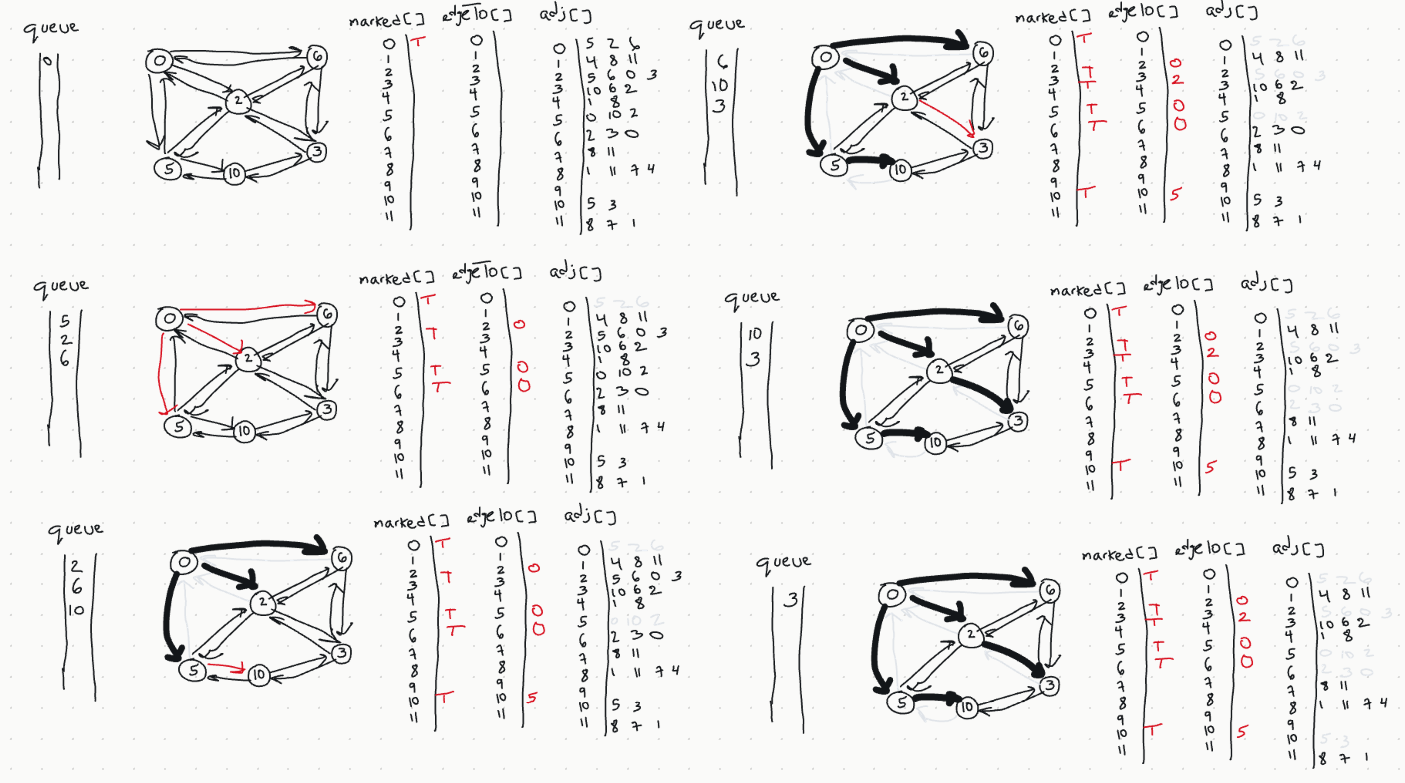
\includegraphics[width=0.9\textwidth]{exercise-11-bfs}
			\caption{Trace of breadth-first search (BFS) on \texttt{tinyGex2.txt}.}
			\label{fig:ex-11-bfs}
		\end{figure}
	\end{sol}
	\begin{sol}
		\begin{figure}
			\centering
			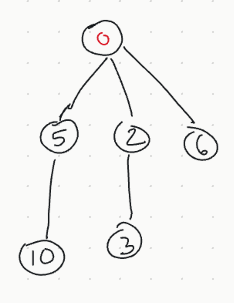
\includegraphics[width=0.2\textwidth]{exercise-11-tree}
			\caption{Tree representation of \texttt{edgeTo[]} array corresponding to
				BFS in Figure~\ref{fig:ex-11-bfs}.}
			\label{fig:ex-11-tree}
		\end{figure}
	\end{sol}
	\begin{ex}{12}
		What does the BFS tree tell us about the distance from \texttt{v} to
		\texttt{w} when neither is at the root?
	\end{ex}
	\begin{sol}
		If the path from the root \texttt{s} to \texttt{v} has length $k$ and
		the path from \texttt{s} to \texttt{w} has length $m$, then it tells us
		that the distance from \texttt{v} to \texttt{w} is bounded by $k + m$, or:
		\begin{align*}
			\text{dist}(\texttt{v},\texttt{w}) \leq \text{dist}(\texttt{v}, \texttt{s})
			+\text{dist}(\texttt{s}, \texttt{w})
		\end{align*}
		However, it does not tell us what the distance is, since we only
		know information about vertices relative to the root \texttt{s}.
	\end{sol}
	\begin{ex}{13}
		Add a \texttt{distTo()} method to the \texttt{BreadthFirstPaths} API and implementation,
		which returns the number of edges on the shortest path from the source to a given
		vertex. A \texttt{distTo()} query should run in constant time.
	\end{ex}
	\begin{sol}
		See \texttt{com.segarciat.algs4.ch4.sec1.ex13}.
	\end{sol}
	\begin{ex}{14}
		Suppose you use a stack instead of a queue when running breadth-first search.
		Does it still compute shortest paths?
	\end{ex}
	\begin{sol}
		No. In Figure ~\ref{fig:ex-14}, if \texttt{0} were the source vertex, and
		\texttt{2} was the last note in the adjacency list for node \texttt{0},
		then it would be the first removed from the stack. Processing it would lead to
		a path of length \texttt{4}, namely \texttt{0-2-5-6-4}, but the shortest path
		from \texttt{0} to \texttt{4} is \texttt{0-1-4}, of length 2.
		\begin{figure}
			\centering
			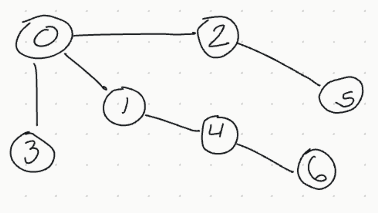
\includegraphics[width=0.3\textwidth]{exercise-14}
			\caption{Exercise 14}
			\label{fig:ex-14}
		\end{figure}
	\end{sol}
	\begin{ex}{15}
		Modify the input stream constructor for \texttt{Graph} to also allow adjacency
		lists from standard input (in a manner similar to \texttt{SymbolGraph}), as in
		the example \texttt{tinyGadj.txt} shown at right. After the number of vertices
		and edges, each line contains a vertex and its list of adjacent vertices.
	\end{ex}
	\begin{sol}
		See \texttt{com.segarciat.algs4.ch4.sec1.ex15}.
	\end{sol}
	\begin{ex}{16}
		The \emph{eccentricity} of a vertex \texttt{v} is the length of the shortest path
		from that vertex to the furthest vertex from \texttt{v}. The \emph{diameter} of a
		graph is the maximum eccentricity of any vertex. The \emph{radius} of a graph is the
		smallest eccentricity of any vertex. A \emph{center} is a vertex whose eccentricity is
		the radius. Implement the following API:
		
		\begin{lstlisting}[language={}]
public class GraphProperties
       GraphProperties(Graph G)    // constructor (exception if G not connected)
	int diameter()                  // diameter of G
	int radius()                    // radius of G
	int center()                    // a center of G	
		\end{lstlisting}

	\end{ex}
	\begin{sol}
		See \texttt{com.segarciat.algs4.ch4.sec1.ex16}.
	\end{sol}
	\begin{ex}{17}
		The \emph{Wiener index} of a graph is the sum of the lengths of the shortest
		paths between all pairs of vertices. Mathematical chemists use this
		quantity to analyze \emph{molecular graphs}, where vertices correspond to
		atoms and edges correspond to chemical bonds. Add a method \texttt{wiener()}
		to \texttt{GraphProperties} that returns the Wiener index of a graph.
	\end{ex}
	\begin{sol}
		See \texttt{com.segarciat.algs4.ch4.sec1.ex17}.
	\end{sol}
	\begin{ex}{18}
		The \emph{girth} of a graph is the length of its shortest cycle. If a graph is
		acyclic, then its girth is infinite. Add a method \texttt{girth()} to
		\texttt{GraphProperties} that returns the girth of the graph. \emph{Hint}: Run
		\texttt{BFS} from each vertex. The shortest cycle containing \texttt{s} is an
		edge between \texttt{s} and some vertex \texttt{v} concatenated with a shortest
		path between \texttt{s} and \texttt{v} (that doesn't use edge \texttt{s-v}).
	\end{ex}
	\begin{sol}
		See \texttt{com.segarciat.algs4.ch4.sec1.ex18}.
	\end{sol}
	\begin{ex}{19}
		Show, in the style of the figure on page 545, a detailed trace of \texttt{CC}
		for finding the connected components in the graph built by \texttt{Graph}'s
		input stream constructor for the file \texttt{tinyGex2.txt} (see \textbf{Exercise 4.1.2}
		and Figure~\ref{fig:tinyGex2-graph}).
	\end{ex}
	\begin{sol}
		See Figure~\ref{fig:ex-19}.
		\begin{figure}
			\centering
			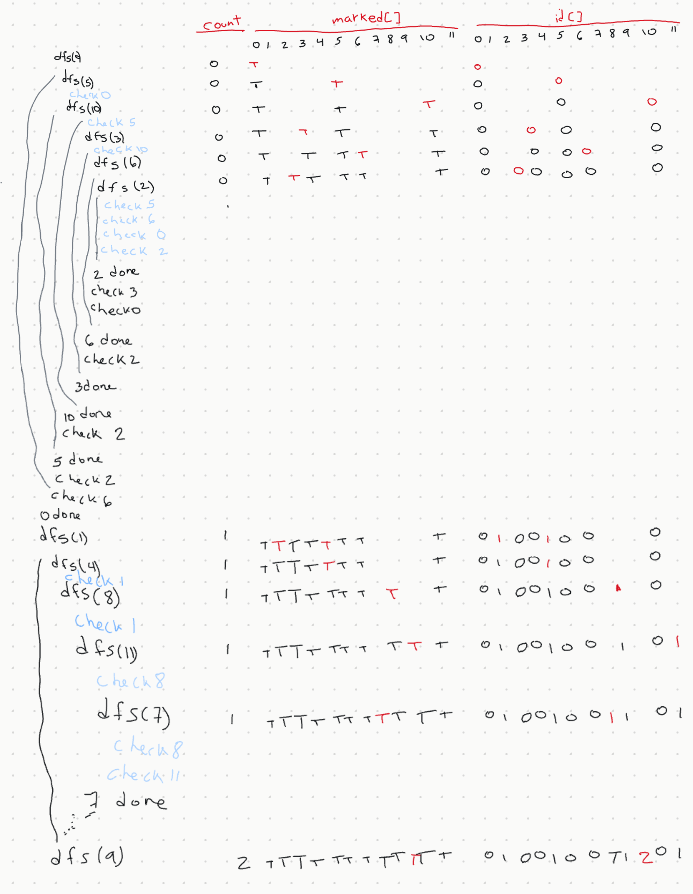
\includegraphics[width=0.8\textwidth]{exercise-19.png}
			\caption{Trace of \texttt{CC} to find the connected components corresponding
			to \texttt{tinyGex2.txt} in \textbf{Exercise 4.1.2}.}
			\label{fig:ex-19}.
		\end{figure}
	\end{sol}
	\begin{ex}{20}
		Show, in the style of the figures in this section, a detailed trace of
		\texttt{Cycle} for finding a cycle in the graph built by \texttt{Graph}'s
		input stream constructor for the file \texttt{tinyGex2.txt} (see \textbf{Exercise 4.1.2}
		and Figure~\ref{fig:tinyGex2-graph}). What is the order of growth of the running time
		of the \texttt{Cycle} constructor, in the worst case?
	\end{ex}
	\begin{sol}
		See Figure~\ref{fig:ex-20}.
		\begin{figure}
			\centering
			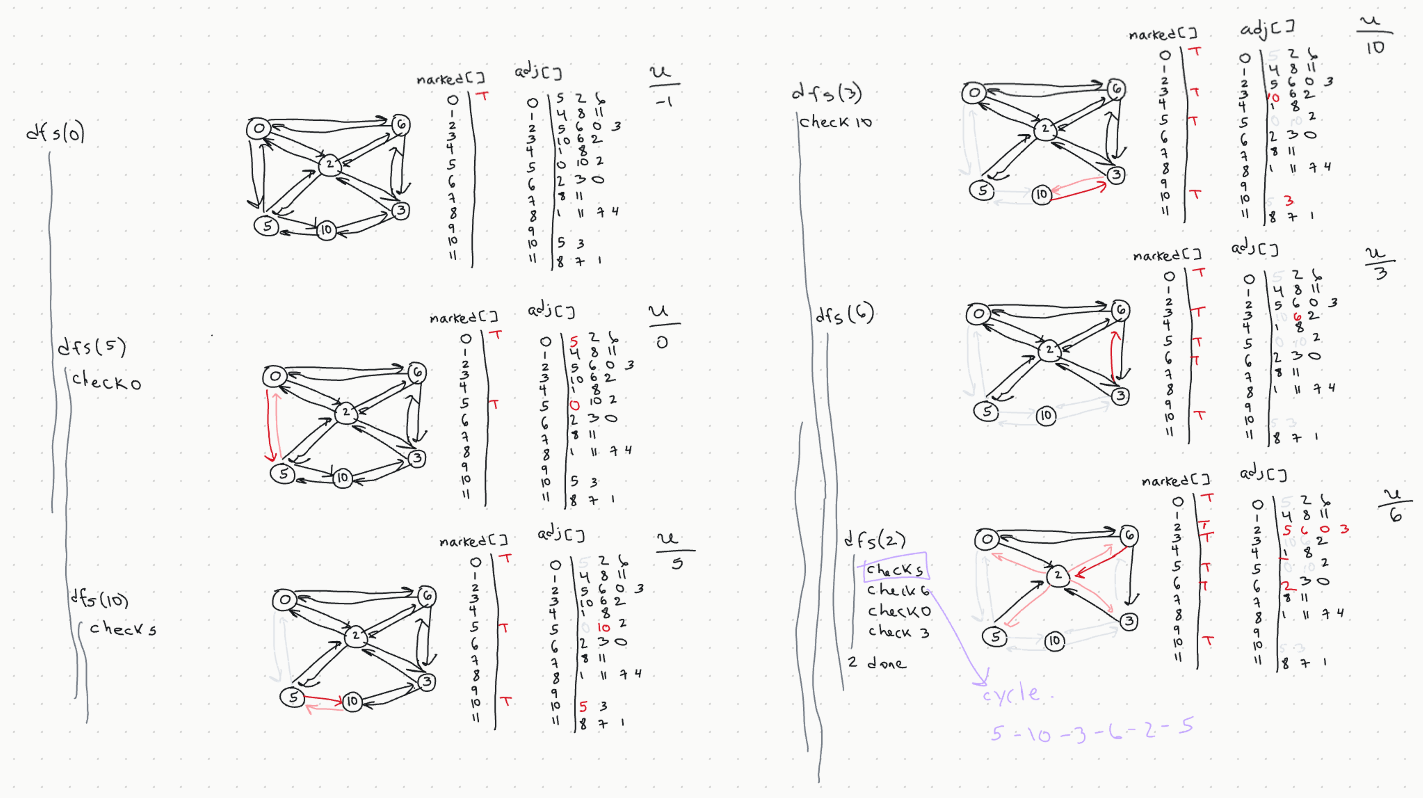
\includegraphics[width=1.00\textwidth]{exercise-20.png}
			\caption{Trace of \texttt{Cycle} to detect a cycle in the graph determined by
				\texttt{tinyGex2.txt} in \textbf{Exercise 4.1.2}.}
			\label{fig:ex-20}.
		\end{figure}
		The constructor of \texttt{Cycle} uses depth-first search on all vertices,
		and its implementation is nearly equivalent to \texttt{CC}.
		Similar to \textbf{Proposition C} in \cite{sedgewick_wayne}, each adjacency-list
		entry is examined once, an all $2E$ entries are examined. Then there is the
		cost for initializing the \texttt{marked[]} array of size $V$. Thus the
		order of growth of the running time of the \texttt{Cycle} constructor is $E+V$
		in the worst case.
	\end{sol}
	\begin{ex}{21}
		Show, in the style of the figures in this section, a detailed trace of
		\texttt{TwoColor} for finding a two-coloring of the graph built by \texttt{Graph}'s
		input stream constructor for the file \texttt{tinyGex.2.txt} (see \textbf{Exercise 4.1.2}
		and Figure~\ref{fig:tinyGex2-graph}). What is the order of growth of the running
		time of the \texttt{TwoColor} constructor, in the worst case?
	\end{ex}
	\begin{sol}
		Once again, the code is similar to \texttt{CC}, applying depth-first search on
		all vertices in the graph. Thus, the order of growth of the running time
		that is about $E+V$ in the worst case, according to \textbf{Proposition C}
		in \cite{sedgewick_wayne}. I am omitting the detailed trace, but upon reaching
		vertex \texttt{2}, and examining its adjacency list, the algorithm would encounter
		vertex \texttt{5} with the same color. Thus the graph is not bipartite.
	\end{sol}
	\begin{ex}{23}
		Write a program \texttt{BaconHistogram} that prints a histogram of Kevin Bacon numbers,
		indicating how many performers from \texttt{movies.txt} have a Bacon number of $0,
		1, 2, 3,\ldots$. Include a category for those who have an infinite number (not connected
		to Kevin Bacon).
	\end{ex}
	\begin{sol}
		See \texttt{com.segarciat.algs4.ch4.sec1.ex23}.
	\end{sol}
	\begin{ex}{24}
		Compute the number of connected components in \texttt{movies.txt}, the size of the
		largest component, and the number of components of size less than 10. Find
		the eccentricity, diameter, radius, a center, and the girth of the largest
		component in the graph. Does it contain Kevin Bacon?
	\end{ex}
	\begin{sol}
		See \texttt{com.segarciat.algs4.ch4.sec1.ex24}.
	\end{sol}
	\begin{ex}{26}
		Write a \texttt{SymbolGraph} client like \texttt{DegreesOfSeparation} that uses \emph{depth-first} search instead of breadth-first search to find paths connecting
		two performers.
	\end{ex}
	\begin{sol}
		See \texttt{com.segarciat.algs4.ch4.sec1.ex26}.
	\end{sol}
	\begin{ex}{27}
		Determine the amount of memory used by \texttt{Graph} to represent a graph with
		$V$ vertices and $E$ edges, using the memory-cost model of Section 1.4
	\end{ex}
	\begin{sol}
		The breakdown is: 16 bytes of object overhead, 4 bytes for the \texttt{int}
		instance variable $V$, 4 bytes for the \texttt{int} instance variable $E$,
		$8$ bytes for the reference to \texttt{adj}, $24$ bytes for the array \texttt{adj},
		itself, making up the flat cost part of $56$ bytes. Next, there are $8V$ bytes of
		references to \texttt{Bag} objects. For each \texttt{Bag} object, there's $16$ bytes
		of overhead, $8$ bytes for the reference to the \texttt{first} node, $4$ bytes
		for a reference to an \texttt{int} for the size, and $4$ bytes of padding.
		That means a $40V$ cost for the \texttt{Bag} objects. Lastly, the cost of each
		\texttt{Node} is about $40$ bytes, of which there are $2E$.
		16 bytes of object overhead, 8 bytes for a reference to the \texttt{item}
		field, 8 bytes for a reference to the \texttt{next} field, 8 bytes for a reference
		to the enclosing class, which is 40 bytes. The referenced object is an \texttt{Integer}, which
		takes up about 24 bytes. Since there are $2E$ values among all adjacency lists
		(since edges are double counted), and each takes about 64 bytes, that comes out to
		$64\cdot 2E=128E$ bytes. The total cost is $56 + 40V + 128E$ bytes.
	\end{sol}
	\begin{ex}{29}
		Modify \texttt{Cycle} so that it works even if the graph contains self-loops and
		parallel edges.
	\end{ex}
	\begin{sol}
		See \texttt{com.segarciat.algs4.ch4.sec1.ex29}.
	\end{sol}
	\begin{ex}{30}
		\emph{Eulerian and Hamiltonian cycles}. Consider the graphs defined by the
		following four sets of edges:
		\begin{lstlisting}[language={}]
0-1 0-2 0-3 1-3 1-4 2-5 2-9 3-6 4-7 4-8 5-8 5-9 6-7 6-9 7-8
0-1 0-2 0-3 1-3 0-3 2-5 5-6 3-6 4-7 4-8 5-8 5-9 6-7 6-9 8-8
0-1 1-2 1-3 0-3 0-4 2-5 2-9 3-6 4-7 4-8 5-8 5-9 6-7 6-9 7-8
4-1 7-9 6-2 7-3 5-0 0-2 0-8 1-6 3-9 6-3 2-8 1-5 9-8 4-5 4-7
		\end{lstlisting}
		Which of these graphs have Eulerian cycles (cycles that visit each edge
		exactly once)? Which of them have Hamiltonian cycles (cycles that visit each
		vertex exactly one)? Develop a linear-time DFS-based algorithm to determine
		whether a graph has a Eulerian cycle (and if so, find one).
	\end{ex}
	\begin{sol}
		To get some geometric intuition, I draw these graphs (though I did not
		include the figures here).
		
		The first graph has a Hamiltonian cycle, but not a Eulerian cycle:
		\begin{lstlisting}[language={}]
# Hamiltonian cycle for first graph:
0-2 2-9 9-5 5-8 8-4 4-7 7-6 6-3 3-1 1-0
		\end{lstlisting}
		The second graph has a Eulerian cycle, but not a Hamiltonian cycle:
		\begin{lstlisting}[language={}]
# Eulerian cycle for second graph:
# edges
0-2 2-5 5-8 8-8 8-4 4-7 7-6 6-9 9-5 5-6 6-3 3-1 1-0 0-3 3-0
# sequence of vertices implied by edges
0-2-5-8-8-4-7-6-9-5-6-3-1-0-3-0
		\end{lstlisting}
		The third graph has a Hamiltonian cycle, but not a Eulerian cycle:
		\begin{lstlisting}[language={}]
# Hamiltonian cycle for third graph:
0-4 4-8 8-7 7-6 6-9 9-5 5-2 2-1 1-3 3-0
		\end{lstlisting}
		The fourth graph has a Hamiltonian cycle, but not a Eulerian cycle:
		\begin{lstlisting}[language={}]
# Hamiltonian cycle for fourth graph:
4-7 7-9 9-3 3-6 6-2 2-8 8-0 0-5 5-1 1-4
		\end{lstlisting}
		After working through the examples, I conjectured that in order for
		a Eulerian cycle to exist, the graph must be connected, and all vertices
		must be of even degree. For example, suppose a vertex $v$ in a graph has
		degree three, and that there was a Eulerian cycle starting at that vertex.
		The cycle must use one of the edges to leave $v$, and one edge to return
		to $v$ at the end. The third edge must be traversed by the definition
		of a Hamiltonian cycle. However, if we used it to enter $v$ at any
		point, then we will have only one edge remaining unused. Since
		a cycle is a path, and paths do not allow repeated edges, we must
		traverse the unused edge. At that point, no unused edge remains to
		return to $v$, and we must accept that there's a contradiction:
		our cycle was not a Eulerian cycle. Since a cycle can be seen from
		the perspective of any vertex, this means that \emph{all} vertices must
		be of even degree for a Eulerian cycle to exist.
	\end{sol}
	\begin{ex}{38}
		\emph{Nonrecursive depth-first search}. Implement depth-first search using an
		explicit stack instead of recursion. \emph{Warning}: Replacing the queue in
		\texttt{BreadthFirstPaths} with a stack yields some graph searching algorithm
		but not depth-first search.
	\end{ex}
	\begin{sol}
		See \texttt{com.segarciat.algs4.ch4.sec1.ex38}.
	\end{sol}
	\pagebreak
	\printbibliography
\end{document}